\documentclass[10pt,a4paper]{article}


% Packages laden
\usepackage[a4paper,top=3cm,bottom=2cm,left=2cm,right=2cm]{geometry}		% paginagrootte
%\usepackage{a4wide}
\usepackage{parskip}									% andere regels voor nieuwe paragraaf: witregel + niet inspringen

\usepackage[english]{babel}						%	spelling en woordafbreking (Engles)
\usepackage[latin1]{inputenc}					% invoer van speciale tekens (bvb. Umlaut)
\usepackage[T1]{fontenc}							% weergave van speciale tekens (bvb. Umlaut)
\usepackage{lmodern}									% betere weergave van speciale tekens (bvb. Umlaut)
\usepackage{dsfont}	
\usepackage{amsfonts,amsthm, tabularx}					% wiskundige symbolen and table of equations
%\usepackage[fleqn]{amsmath}

% Package for hyperlink, without ugly box around and nice blue color for text
\usepackage{hyperref}
\usepackage{xcolor}
\hypersetup{
    colorlinks,
    linkcolor={red!50!black},
    citecolor={blue!50!black},
    urlcolor={blue!80!black}
}

\usepackage{graphicx}
\usepackage{caption}
\usepackage{subcaption}

\usepackage{float}										% plaatsen van figuren en tabellen
\usepackage[format=plain,
						indent=1cm]{caption}			% personaliseren van onderschriften
\usepackage{eurosym}									% sign of euro

% Instellingen voor document
\renewcommand{\arraystretch}{1.1}			% tabelrijen iets hoger maken

\usepackage[squaren,Gray]{SIunits}
\usepackage{amsmath,amsfonts,amsthm,mathrsfs,MnSymbol}	% wiskundige symbolen
\renewcommand*\thesection{\arabic{section}}
\DeclareMathOperator*{\argmin}{\arg\!\min}
\usepackage{pifont}							

\setcounter{secnumdepth}{3}		% Enable subsubsection numbering
\setcounter{tocdepth}{3}		% Include subsubsection in table of content

\usepackage{color}				% Load the color package: \color{declared-color}{text}. If also background:
								% \colorbox{declared-color1}{\color{declared-color2}text}
%Aangepaste header
\usepackage{fancyhdr}
\pagestyle{fancyplain}
\renewcommand{\headrulewidth}{1.0pt}
\lhead{\fancyplain{}{Crash course modelica}}
\rhead{\fancyplain{}{12 oct. 2015}}

\author{Damien Picard}
						
\begin{document}

\section*{Exercise 1}
The purpose of this exercise is to model an electrical circuit using only your own code implementation. You will learn how to create connectors, partial models, models and how to re-use your code.

\begin{figure}[h]
\centering
\begin{minipage}{.5\textwidth}
  \centering
  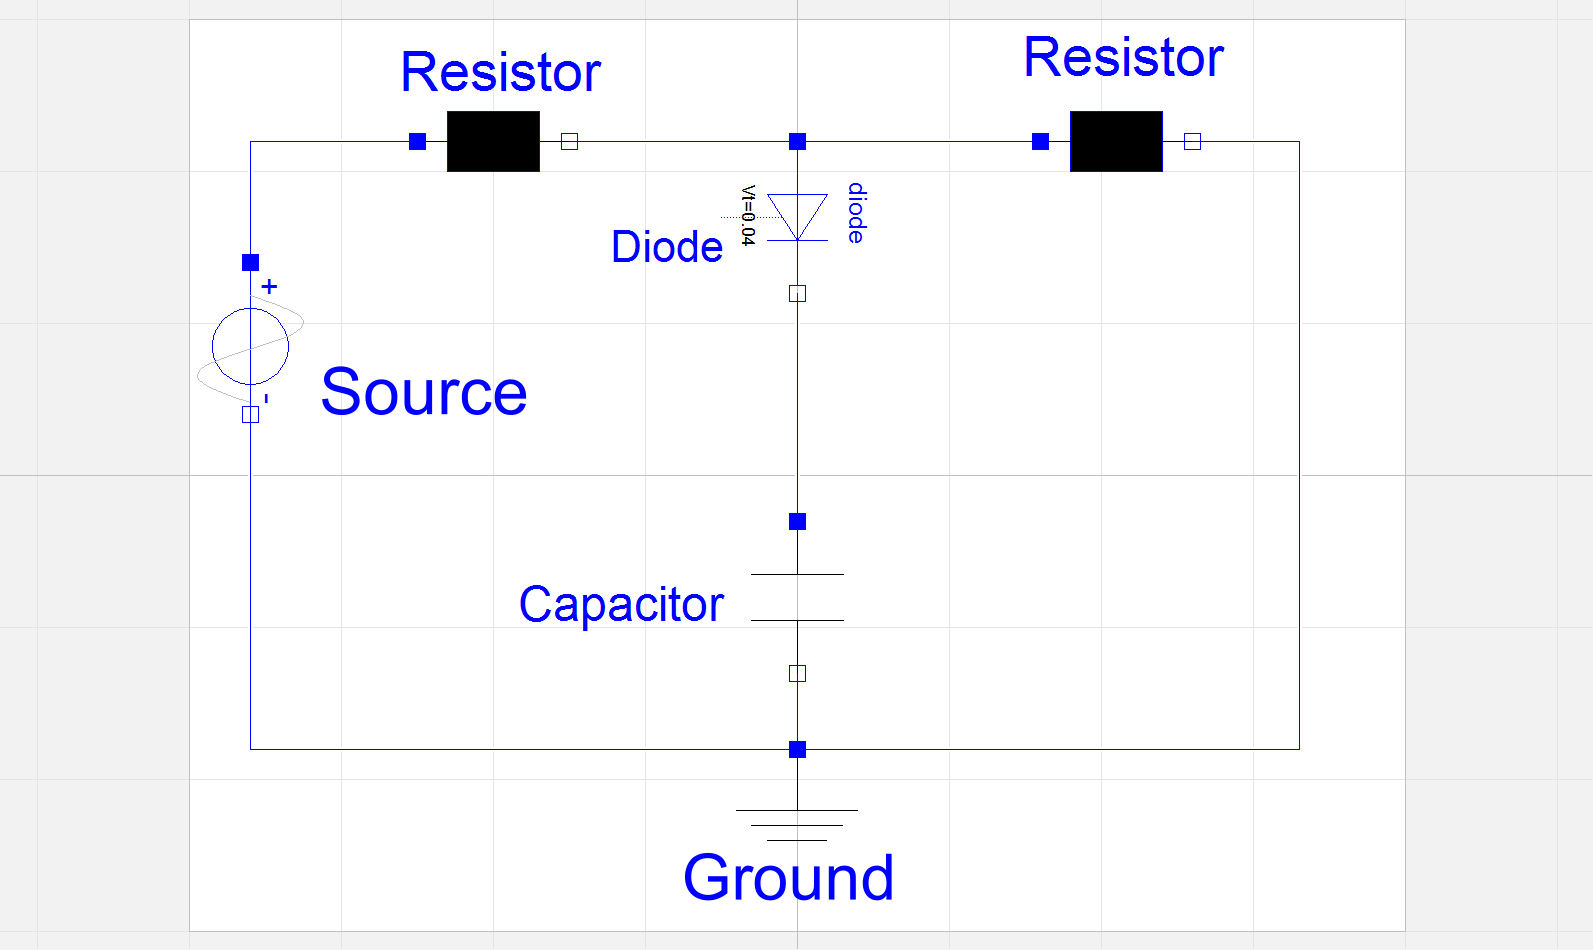
\includegraphics[width=1\linewidth]{Figures/circuit.png}
  \captionof{figure}{Electrical circuit.}
  \label{fig:cir}
\end{minipage}%
\begin{minipage}{.5\textwidth}
  \centering
  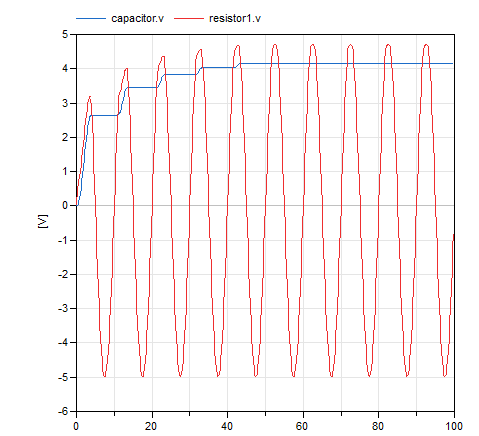
\includegraphics[width=.8\linewidth]{Figures/result.png}
  \captionof{figure}{Result of simulation}
  \label{fig:res}
\end{minipage}
\end{figure}


Consider the electrical circuit depicted in Fig. \ref{fig:cir}. It is composed of a sinusoidal source, a resistor, a diode, a capacitor and the ground. Create this circuit from scratch by following the following steps:


\begin{enumerate}
\item Create a new \textit{package} called \textit{MyLib}
\item Each component uses electrical connectors. Create a partial connector called \textit{Pin} which contains the variables $i$ (current) and $v$ (voltage). Which is a \textit{flow} and which is a \textit{potential} variable? Create then the connectors \textit{Pin\_a} and \textit{Pin\_b} for the positive and negative pins. Make two different graphical illustrations for the pins.
\item Create a partial model \textit{OnePin} which contains the variables $i$ (current) and $v$ (voltage) and a connector \textit{Pin\_a}. This model will later be extended by all \textit{OnePin} component. Create also a partial model \textit{TwoPin} with the same variables and two \textit{Pin} connectors. The variable \textit{v} should give the voltage drop between the two pins and the variable \textit{i} the current between them. Be careful with the sign of \textit{i}!
\item Create the source, the resistor, the diode and the capacity by extending \textit{OnePin} or \textit{TwoPin}. Make use of the following equations:
\begin{enumerate}
\item Resistor: $R i_{1 \rightarrow 2} = v_1 - v_2$
\item Capacity: $C \frac{d v}{dt} = i$
\item source: $v = V sin( 2 \pi f t + \omega) + \beta$
\item diode: if $ \frac{v}{V_t} \geq \alpha$: $i = I_{ds} ( e^\alpha ( 1 + \frac{v}{V_t} - \alpha) - 1) + \frac{v}{R}$, else $i = I_{ds} (e^\alpha - 1) + \frac{v}{R}$
\item ground: $ v = 0$
\end{enumerate}
Make use of following values for the diode: $I_{ds}$ = 1.e-6, $V_t=0.04$, $\alpha=15$, $R=1.e8$.
\item Create a model called \textit{Circuit} which combined all these components.
\item Simulate the circuit for 100 seconds.
\end{enumerate}





\end{document}
